\chapter{Introduction}

The Internet was created with the idea that any two computers connected to the common network should be able to communicate with each other. In \textit{Internet Protocol version 4 (IPv4)} which routes most traffic today, each computer gets assigned an address which is subsequently used for packet routing. As IPv4 uses a 32-byte address space, it is not feasible to assign a unique address to every device on the planet. To deal with IPv4 address exhaustion, internet providers were forced to deploy \textit{Network Address Translation (NAT)}, which allows a single address to be shared across multiple devices behind a NAT device.

Another issue appeared with the rise of portable computers and smartphones. IPv4 addresses are dependent on the physical location and can not be in any way considered as stable user identifiers. There has been several proposals including Mobile IP, IPSec, and IPv6 to improve the usability and security of the Internet Protocol. However, none of them have been widely deployed yet or address all known issues.

This thesis proposes and implements a decentralized protocol for peer to peer communication. The protocol allows any two devices to establish a direct connection by taking advantage of NAT traversal techniques to connect to peers behind NATs. When the Internet connection is not available and peers are located in proximity, the connection can be established using Bluetooth. Peers are addressed by their public keys and their physical addresses on lower layers are abstracted away.

The protocol makes best effort to connect peers behind NATs. In case the connection is not possible, it resorts to a relay protocol. Bandwidth accounting prevents misusing the relay servers and provides incentive for relay operators. The protocol is completely decentralized and does not rely on any central entity.

%This also allows to route messages over multiple transports. For example, a message can be send over Bluetooth and delivered to a user connected over the Internet by using another device a relay.

To show one of many practical use cases of the protocol, a simple chat messaging application is implemented on top of it. It allows to send not only text messages, but also images and videos to demonstrate binary file transfer.

Compared to the state of the art solutions, it combines both nearby and Internet connectivity, does not require any central server, and is completely open source. Finally, the protocol performance is experimentally evaluated with multiple Android devices connected to different Wi-Fi and carrier networks and running a stress test over the period of 24 hours.

\iffalse
\fi

\chapter{Problem Description}

\section{Ubiquitous Overlay Network}



% history of internet, IPv4
% address exhaustion, mobility

% NAT breaks end-to-end principle
% solutions:
% - IPv6
% - Mobile IP
% - IPSec
% IPv6 still not widely deployed
% - TU preparing for IPv6 since 2012
% - not available on any cellular network in NL

% motivation for decentralized internet
% problems with current internet:
% - censorship
% - data in control of big companies
% we need building blocks to disrupt centralized services
% data in controls of users
% first steps: connectivity, data availability, privacy
% mention blockchain as enabler of permissionless economic activity

% ubiquitous overlay
% - peer to peer connectivity over the Internet
% - off-grid communication without internet access
% -

\section{Network Address Translation}

\subsection{NAT Classification}

\subsection{Carrier Grade NAT}

\subsection{Port Forwarding}

% mention protocols for port forwarding configuration: UPnP-IGD, NAT-PMP, PCP
% usually not enabled by default, not enabled in carrier networks

\section{Nearby Communication}

Modern smartphone devices come equipped with several wireless communication standards that can potentially be used for communication with other nearby devices. It is desirable to use such a technology when multiple devices in proximity want to communicate with each other when there is no reliable Internet infrastructure available. These technologies can be also preferred over the Internet in case of censorship and privacy concerns, as has been shown during numerious occasions such as Hong Kong protests. From the user experience perspective, it is desired that the device discovery and connection establishment does not require any user interaction besides the one required by the application use case. However, this is often opposed by the security model of smartphone operating systems which try to protect users by enforcing system UI for any sensitive operations.

Probably the oldest and the most battle-tested technology is Bluetooth, which has been in development for over more then 20 years already. The common flow for Bluetooth usage is to first force user to pair two devices. Only then, \textit{Radio frequency communication (RFCOMM)} channel can be established between paired devices. This process requires user interaction which degrades the user experience in certain applications when authentication is performed on the application level. While it is possible to establish an \textit{insecure} RFCOMM channel if the MAC address of the other device is known, the user of the other device still needs to manually set it to be \textit{discoverable}.

In Bluetooth 4.0 standard, \textit{Bluetooth Low Energy (BLE)} has been introduced. It is a completely different communication protocol incompatible with the classic Bluetooth, which we will further refer to as \textit{Bluetooth Classic}. Compared to Bluetooth Classic, BLE offers considerably decreased power consumption with a similar communication range. Its was originally intended to support an infrequent low-power communication with wearables, healthcare accessories, or smart home appliances. However, while it is not a primary use case, it could also be potentially used for low-bandwidth peer-to-peer communication between smartphone devices. It is notable that once user allows Bluetooth permission, the application can fully control BLE APIs without any user interaction, which opens up doors for a range of many different applications.

% technologies available on smartphones:
% - Bluetooth, BLE, WiFi Direct, WiFi Aware
% infrastructureless communication

% Bluetooth Classic
% - requires the device to be discoverable - user interaction
% - no interoperability between iOS and Android
% Bluetooth Low Energy
% - energy efficient, does not require pairing, but lower bandwidth
% - API on Android very low level, error-prone to use
% - role simultaneity – master and slave at the same time

\section{Peer Discovery}


\chapter{State of the Art}

\section{NAT Traversal}

\subsection{Session Traversal Utilities for NAT (STUN)}

\subsection{Traversal Using Relays around NAT (TURN)}

\subsection{Interactive Connectivity Establishment (ICE)}

\subsection{ICMP Hole Punching}

\subsection{Symmetric NAT Traversal}

\section{P2P Communication Libraries}

\subsection{libp2p}

\subsection{IPv8}

\subsection{Nearby Connections API}

\subsection{Bridgefy SDK}

\chapter{Design}

%\section{NAT Detection}

\section{NAT Traversal with Peer Introductions}

%\section{Port Forwarding}

%\section{Symmetric NAT Traversal}

% \section{Network Service Discovery}

\section{Relay Protocol with Bandwidth Accounting}

\section{Nearby Communication over Bluetooth}

%\subsection{Bluetooth Low Energy}

%\subsection{Roles in BLE}

%\subsection{Generic Attribute Profile}

%\subsection{Using Bluetooth Low Energy for P2P Communication}

\begin{figure}
    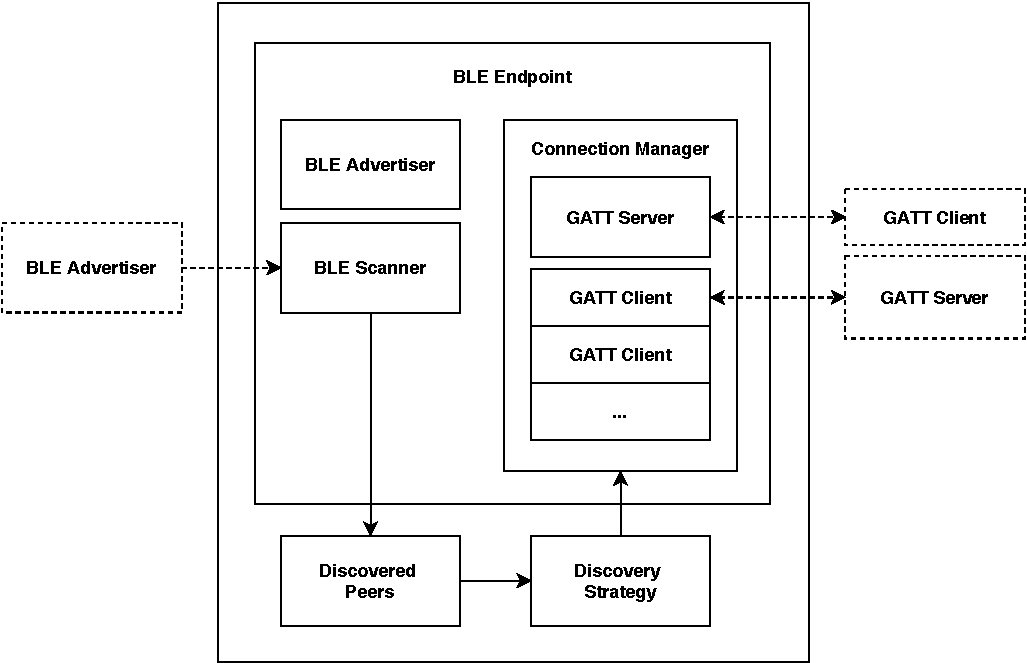
\includegraphics[width=\textwidth]{diagrams/bluetooth-architecture}
    \caption{Bluetooth Low Energy Communication Architecture}
\end{figure}

\subsection{BLE Advertising}

\subsection{BLE Scanning}

\subsection{GATT Server}

\begin{figure}
    \centering
    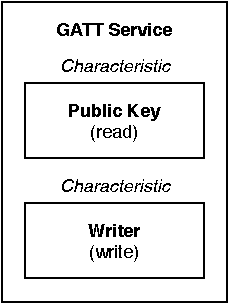
\includegraphics[width=0.25\textwidth]{diagrams/bluetooth-gatt}
    \caption{GATT Server Architecture}
\end{figure}

\subsection{Discovery Strategy}

% GATT - service, characteristic, descriptor
% Service IPv8
% Characteristics
% - Member ID, permission read
% - Writer, permission write
% Handshake
% - 1. Read Member ID
% - 2. Wait for other peer to read our Member ID
% - 3. Send data to peer via its Writer

% Future Work:
% - L2CAP connection oriented channels (Android 10+)

% https://medium.com/@martijn.van.welie/making-android-ble-work-part-3-117d3a8aee23
% https://stefanbossbaly.com/2018/08/06/ble-in-android
% https://blog.classycode.com/a-short-story-about-android-ble-connection-timeouts-and-gatt-internal-errors-fa89e3f6a456
% https://punchthrough.com/android-ble-development-tips

\chapter{Implementation}

\section{Project Structure}

% JVM vs. Android
% unit tests, TODO: Android tests
% library vs. super app separation

\section{System Architecture}

\subsection{Communities}

\subsection{Discovery Strategies}

\subsection{Endpoints}

\section{Bootstrap Server}

%\section{Bluetooth Ad-Hoc Network}
%\subsection{Bluetooth Low Energy}
%\subsection{Generic Attribute Profile}

%\section{Multi-Transport Routing Algorithm}

%\section{Peer Discovery and Traversal in Distributed Hash Table}

%\section{Packet Format}

\section{Maintaining Backward Compatibility}
% continuous improvement while maintaining backward compatibility with 10 year old ipv8 implementation

\section{TrustChain Explorer}

\section{Binary Transfer over UDP}

\section{PeerChat: Distributed Messenger}

\section{Testbed for Distributed Android Applications}


\chapter{Experiment}

\section{Analysis and Puncturing of Carrier Grade NAT}

According to the report by Statista \cite{statista:marketshare}, there were three major mobile phone operators providing services in the Netherlands in Q4 2018. They are listed in Table \ref{table_marketshare}. In total, these represent up to 85 \% of the market share. The rest of the market is shared by Mobile Virtual Network Operators who sell services over existing networks of those three operators.

\begin{table}[h!]
    \centering
    \begin{tabular}{ | l | c | }
        \hline
        \textbf{Operator} & \textbf{Market share} \\
        \hline
        KPN & 35\% \\
        Vodafone & 25\% \\
        Mobile Virtual Network Operators & 25\% \\
        T-Mobile & 20\% \\
        \hline
    \end{tabular}
    \caption{Market share of mobile network operators in the Netherlands in Q4 2018. The shares do not sum up to 100\% as they are rounded up within five percent ranges in the original report. \cite{statista:marketshare}}
    \label{table_marketshare}
\end{table}

We have purchased pre-paid SIM cards for all three major mobile network operators to investigate whether they are suitable for peer-to-peer communication. First, we tried to infer the characteristics of their Carrier Grade NAT deployments.

We used the STUN protocol and NAT behavior discovery mechanisms described in \cite{rfc5780}. They have shown that all networks appear to use \textit{Endpoint-Independent Mapping (EIM)} and \textit{Address and Port-Dependent Filtering} (also known as \textit{port-restricted cone NAT}). EIM is a sufficient condition for our NAT traversal mechanism to be successful, so this would make all these NATs suitable for P2P communication.

However, as NAT behavior can change over time, we performed some more tests to verify that the behavior is consistent over time. We attempted to connect to 50 different peers over the interval of 5 minutes. We verified that KPN and T-Mobile networks are consistent with EIM behavior. However, the Vodafone network changes the mapped port for new connections approximately every 60 seconds, even when connecting to the same IP address and a different port. This behavior can be described as \textit{Address and Port-Dependent Mapping}, which is characteristic for a \textit{symmetric NAT}.

The mapped ports seem to be assigned at random from the range of 10,000 ports, which makes it infeasible to use any known symmetric NAT traversal techniques such as port prediction or multiple hole punching \cite{multihole}\cite{takeda}.

%The results are presented in Table \ref{table_cgnat_analysis}.

\iffalse

\begin{table}[h!]
    \centering
    \begin{tabular}{ | l | l | l | l | }
        \hline
        \textbf{Operator} & \textbf{Mapping behavior} & \textbf{Filtering behavior} & \textbf{Binding lifetime} \\
        \hline
        KPN & Endpoint-Independent & Address and Port-Dependent & ? \\
        Vodafone & Endpoint-Independent / Address and Port-Dependent & Address and Port-Dependent & ? \\
        T-Mobile & Endpoint-Independent & Address and Port-Dependent & ? \\
        \hline
    \end{tabular}
    \caption{Characteristics of CGNATs deployed by Dutch mobile network operators}
    \label{table_cgnat_analysis}
\end{table}

\fi

% Types of NAT used by different operators
% - T-Mobile - Address-restricted cone
% - Vodafone – symmetric NAT, random port mapping, TODO: analyze port distribution
% - KPN - Address-restricted cone

\section{Performance Evaluation}

\subsection{Bootstrap Performance}

\subsection{Stress Test}

% experiments:
% - bootstrap from 0 to 20 peers
% - 24-hour stress test


\chapter{Conclusion}

\section{Future Work}
% IPv6 support, multiple network interfaces
